\chapter{Entwurf}
\label{chap:entwurf}

Dieses Kapitel stellt die Architektur von TeamBoard vor. Der Schwerpunkt liegt nicht auf einer vollständigen Aufzählung aller Funktionen, sondern auf den Entwurfsentscheidungen und den Abwägungen, die zu ihnen geführt haben. Für jede zentrale Entscheidung werden die betrachteten Alternativen, der gewählte Weg und der dafür in Kauf genommene Preis benannt.

\section{Vorstellung und Diskussion der gewählten Architektur}
\label{sec:architektur-diskussion}

TeamBoard ist als komponentenbasiertes Microservice-System umgesetzt. Das System besteht aus sieben fachlichen Diensten hinter einem gemeinsamen API-Gateway, ergänzt um einen Protokoll-Adapter für die Anbindung von Sprachmodell-Clients. Die Dienste sind entlang fachlicher Grenzen geschnitten und kommunizieren bevorzugt asynchron über einen zentralen Event-Bus.

Die Architektur folgt zwölf verbindlichen Prinzipien, die in der Architektur-Referenz des Repositorys festgehalten sind. Eine Abweichung von einem Prinzip erfordert einen dokumentierten Architecture Decision Record (ADR). Die folgenden Abschnitte diskutieren die wichtigsten dieser Entscheidungen.

\subsection{Microservices}

Die Aufgabenstellung fordert ausdrücklich ein komponentenbasiertes System mit unabhängig skalierbaren Diensten. Ein modularer Monolith wäre in der Entwicklung und im Betrieb einfacher gewesen und hätte verteilte Transaktionen vermieden. Er hätte jedoch die geforderte unabhängige Skalierung und die klare fachliche Trennung nur eingeschränkt abgebildet. Die Entscheidung fiel daher auf einen Schnitt in eigenständige Dienste. Der Preis dafür ist ein höherer Betriebsaufwand und die Notwendigkeit, Konsistenz über Dienstgrenzen hinweg aktiv zu behandeln.

Der Zuschnitt orientiert sich an Domain-Driven Design. Jeder Dienst bildet einen fachlichen Bounded Context mit eigener Sprache ab. Der Umfang wurde bewusst als tragfähiges Minimum gewählt und lässt sich schrittweise erweitern, statt von Beginn an alle denkbaren Funktionen aufzunehmen.

\subsection{Asynchrone Ereignisse}

Die Dienste tauschen fachliche Ereignisse über einen RabbitMQ-Topic-Exchange aus. Synchrone Aufrufe werden nur dort eingesetzt, wo der Benutzer eine sofortige Antwort benötigt oder ein Dienst eine Information verbindlich zum Zeitpunkt der Aktion braucht. Die betrachtete Alternative war eine durchgehend synchrone Kommunikation über REST. Sie hätte einfachere Nachvollziehbarkeit geboten, aber die Dienste eng gekoppelt und die Verfügbarkeit voneinander abhängig gemacht. Der ereignisgetriebene Ansatz entkoppelt die Dienste, sodass ein neuer Empfänger ohne Änderung am Sender hinzukommt. Als Preis ergibt sich Eventual Consistency nach außen, die durch idempotente Verarbeitung und eine Dead-Letter-Queue abgesichert wird.

\subsection{Database-per-Service}

Jeder Dienst besitzt seine eigene Datenbank und ist die alleinige Datenhoheit für seinen Bereich. Ein direkter Datenbankzugriff zwischen Diensten ist ausgeschlossen. Eine geteilte Datenbank hätte Joins über Fachgrenzen und starke Konsistenz erlaubt, aber die Dienste über das Schema fest gekoppelt und unabhängige Weiterentwicklung erschwert. Die getrennten Datenbanken sichern die Autonomie der Dienste. Der Preis ist, dass fachübergreifende Sichten über Ereignisse oder Schnittstellen zusammengeführt werden müssen und nicht per SQL-Join entstehen.

\subsection{Outbox-Pattern}

Ein Dienst, der eine Datenänderung vornimmt und dazu ein Ereignis veröffentlicht, steht vor dem Problem, dass beide Schritte auseinanderlaufen können. Ein direktes Publizieren nach dem Commit kann ein Ereignis verlieren, wenn der Broker im falschen Moment nicht erreichbar ist. Deshalb schreibt jeder Dienst das Ereignis in derselben Datenbanktransaktion wie die Datenänderung in eine Outbox-Tabelle. Ein gemeinsamer Worker liest diese Tabelle und publiziert die Ereignisse. Die Alternative eines verteilten Zwei-Phasen-Commits wurde wegen ihrer Komplexität und schlechten Skalierbarkeit verworfen. Der Preis der Outbox ist eine geringe zusätzliche Latenz durch das Polling und der Betrieb des Workers.

\subsection{Zero-Trust}

Das Gateway übernimmt Routing, Rate-Limiting und CORS, prüft aber bewusst keine Benutzer-Token. Stattdessen validiert jeder Dienst das JWT selbst gegen den öffentlichen Schlüssel des Auth-Service. Eine zentrale Prüfung am Gateway wäre einfacher zu konfigurieren gewesen, hätte aber eine implizite Vertrauensstellung allein aufgrund der Netzwerklage geschaffen. Der gewählte Zero-Trust-Ansatz macht jeden Dienst unabhängig prüfbar. Interne Aufrufe zwischen Diensten tragen zusätzlich ein kurzlebiges Service-Token. Der Preis ist ein wiederkehrender Validierungsaufwand in jedem Dienst, der durch eine geteilte Bibliothek und einen Schlüssel-Cache gering gehalten wird.

\subsection{Zentrale Autorität für Berechtigungen}

Der Project-Service ist die autoritative Quelle für projektbezogene Berechtigungen. Andere Dienste fragen vor schreibenden Operationen synchron dort an, ob ein Benutzer die Operation ausführen darf. Die Alternative, Berechtigungen in jedem Dienst zu spiegeln, hätte den Synchron-Aufruf vermieden, aber die Gefahr widersprüchlicher Rechtestände erzeugt. Die zentrale Autorität hält die Regeln an einer Stelle konsistent. Der dabei entstehende Synchron-Aufruf wird über einen Redis-Cache mit kurzer Lebensdauer entschärft, der bei Mitgliederänderungen gezielt invalidiert wird.


\section{Architekturübersicht}
\label{sec:architekturbild}

\vref{fig:architektur-gesamt} zeigt das Gesamtsystem mit seinen Komponenten und deren Interaktion. Die Clients erreichen das System ausschließlich über das Gateway. Dahinter liegen die fachlichen Dienste, die untereinander über den Event-Bus und über wenige synchrone Aufrufe kommunizieren. Die Infrastruktur besteht aus einer PostgreSQL-Instanz mit je einer logischen Datenbank pro Dienst, einem Redis für Cache und WebSocket-Backplane, dem RabbitMQ-Event-Bus und einem S3-kompatiblen Objektspeicher für Dokumente.

\begin{figure}[ht]
  \centering
  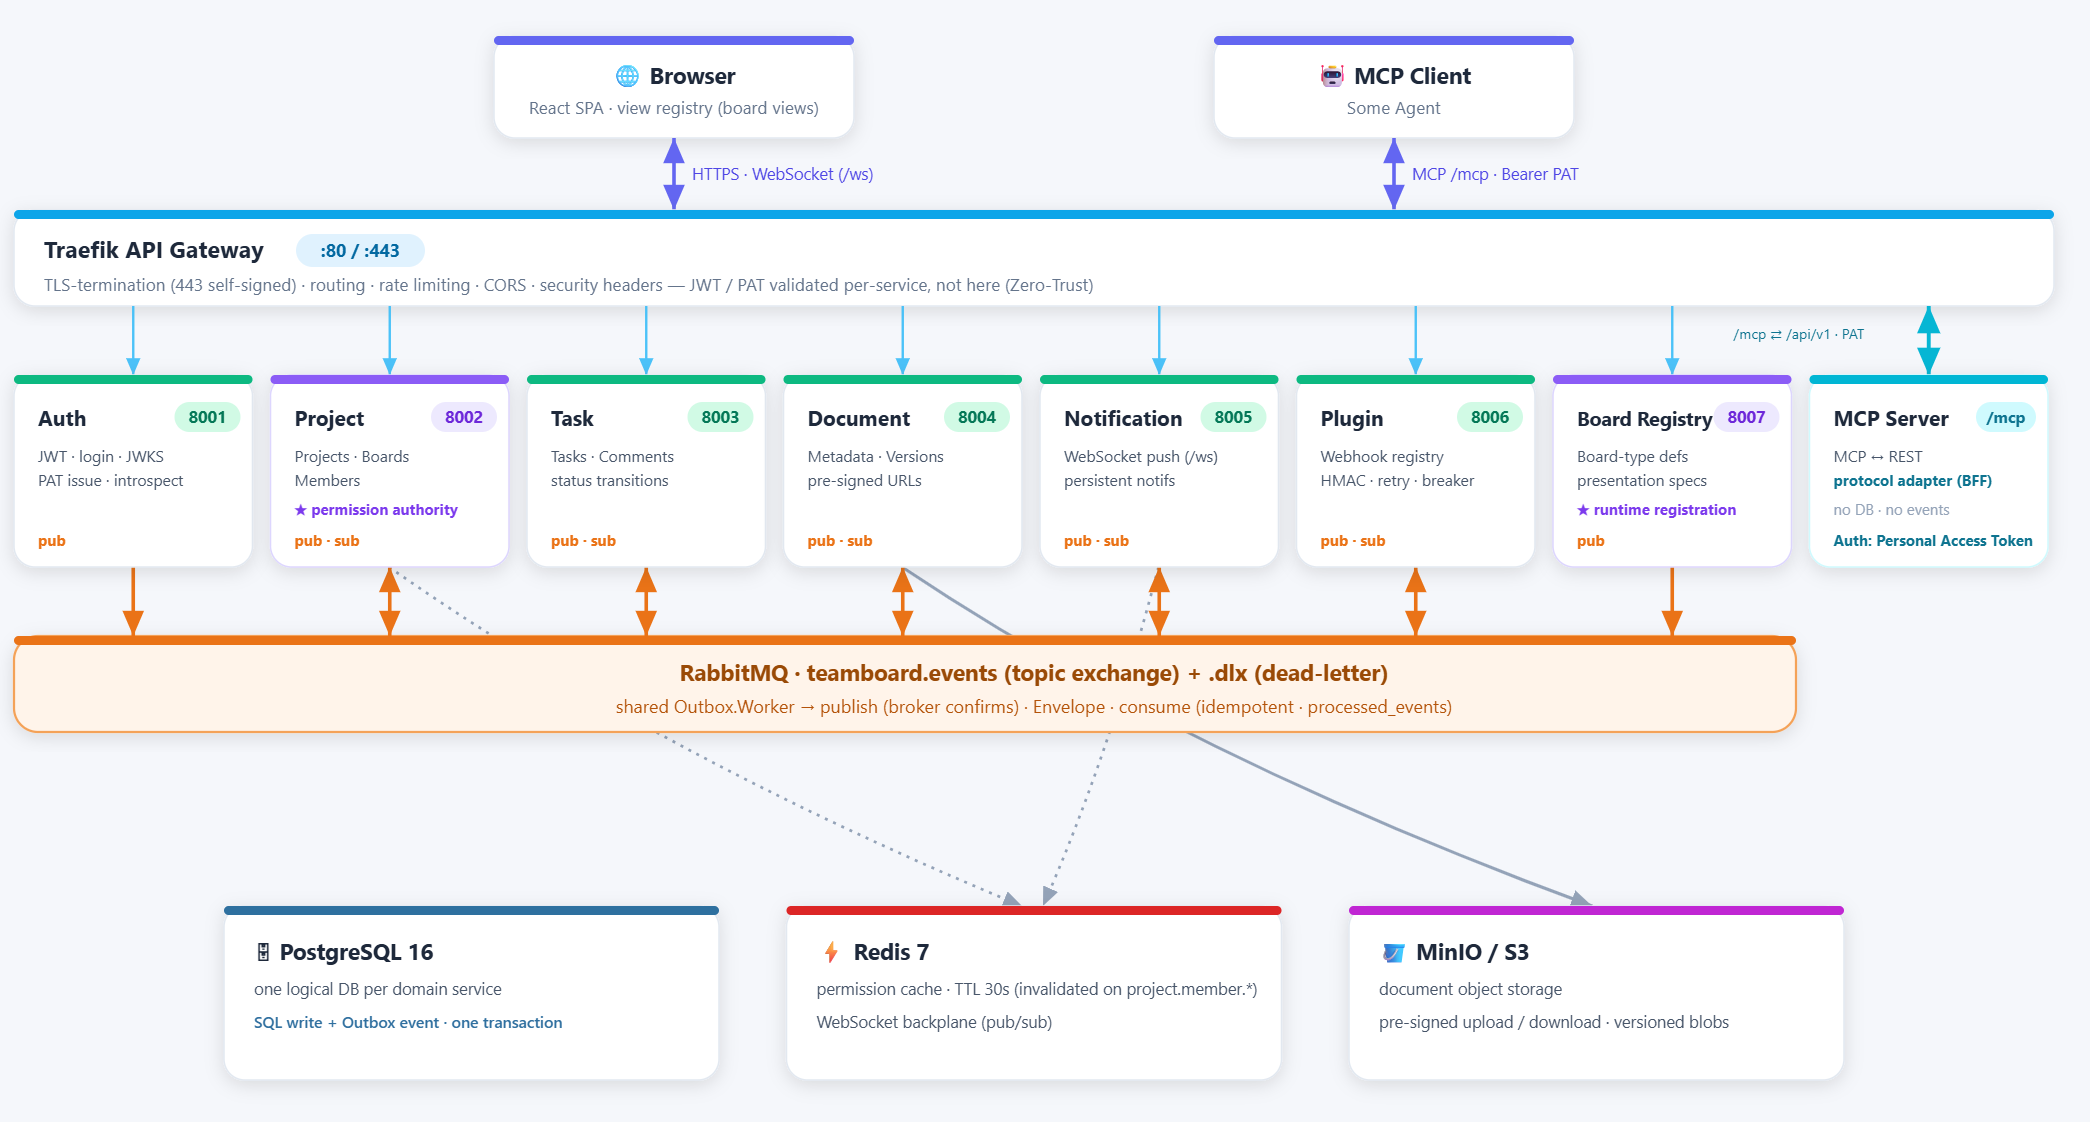
\includegraphics[width=\linewidth]{resources/plots/architecture.png}
  \caption{Gesamtarchitektur von TeamBoard mit Clients, Gateway, Diensten, Event-Bus und Infrastruktur.}
  \label{fig:architektur-gesamt}
\end{figure}

Die Grafik gliedert das System in horizontale Schichten. Ganz oben stehen die Clients, das Web-Frontend und der MCP-Client. Darunter liegt das Traefik-Gateway als einziger Eintrittspunkt, das Token bewusst nicht selbst prüft, sondern die Prüfung jedem Dienst überlässt. Es folgt die Reihe der fachlichen Dienste mit ihren Ports, ergänzt um den MCP-Server am rechten Rand. Darunter zieht sich der RabbitMQ-Event-Bus als gemeinsame Leitung durch das System. Am unteren Rand steht die Infrastruktur aus PostgreSQL, Redis und dem Objektspeicher. Die blauen Pfeile zeigen den Anfragefluss durch das Gateway, die orangen Pfeile das Veröffentlichen und Konsumieren von Ereignissen, die gestrichelten Linien die Anbindung an Cache und Objektspeicher. Die Grafik entstammt der Quelle im Repository unter \path{docs/architecture.svg}.

Drei Merkmale prägen das Bild. Erstens ist das Gateway der einzige Eintrittspunkt, prüft aber selbst keine Token. Zweitens laufen fachliche Ereignisse über den Topic-Exchange, sodass kein Sender seine Empfänger kennt. Drittens hält jeder Dienst seine eigenen Daten, und nur der Notification-Service hält bewusst Zustand in Form offener WebSocket-Verbindungen.

\section{Die einzelnen Komponenten}
\label{sec:komponenten}

Dieser Abschnitt stellt die Komponenten vor. Die fachlich einfacheren Dienste werden knapp beschrieben, die Board Registry und der Plugin-Service sowie der MCP-Server ausführlicher, da ihre Entwurfsentscheidungen für die Erweiterbarkeit des Systems zentral sind.

\subsection{Auth-Service}
\label{sub:auth}

Der Auth-Service verantwortet Identität und Authentifizierung. Er übernimmt Registrierung, Login, Token-Refresh und den Passwort-Reset und stellt signierte JWT aus. Über einen JWKS-Endpunkt veröffentlicht er den öffentlichen Schlüssel, mit dem alle anderen Dienste die Token prüfen. Projektbezogene Rollen gehören ausdrücklich nicht in diesen Dienst. Zusätzlich verwaltet der Auth-Service langlebige Personal Access Tokens für externe Clients und löst sie auf Anfrage anderer Dienste auf.

\subsection{Project-Service}
\label{sub:project}

Der Project-Service verwaltet Projekte, Boards und Mitgliedschaften und ist die autoritative Quelle für Berechtigungen. Er entscheidet über Rollen und deren Rechte und beantwortet die Berechtigungsanfragen der übrigen Dienste. Beim Anlegen eines Boards löst er den gewählten Board-Typ zur Laufzeit über die Board Registry auf und validiert die Board-Konfiguration gegen das vom Typ gelieferte Schema. Die Board-Instanzen bleiben in seiner Hoheit, während die Typ-Definitionen in der Registry liegen.

\subsection{Task-Service}
\label{sub:task}

Der Task-Service verwaltet Aufgaben innerhalb eines Boards mit Statusübergängen, Zuweisungen, Fälligkeiten, Kommentaren und Anhang-Referenzen. Er führt einen Audit-Trail über Änderungen. Den fachlichen Status einer Spalte leitet er nicht mehr aus dem Spaltennamen ab, sondern übernimmt ihn aus den expliziten Status-Angaben, die über Ereignisse aus dem Board-Kontext eintreffen. Vor schreibenden Operationen prüft er die Berechtigung beim Project-Service.

\subsection{Document-Service}
\label{sub:document}

Der Document-Service verwaltet Dokumente als Metadaten mit Verweis auf einen Objektspeicher und unterstützt Versionierung. Die eigentlichen Dateien fließen über vorsignierte URLs direkt zwischen Client und Objektspeicher, sodass der Dienst selbst keine großen Datenmengen durchleiten muss. Jede neue Version erhält einen eigenen Objekt-Schlüssel, was den Zugriff auf frühere Stände erlaubt.

\subsection{Notification-Service}
\label{sub:notification}

Der Notification-Service liefert Echtzeit-Benachrichtigungen über WebSockets und speichert persistente Benachrichtigungen. Er ist die einzige bewusst zustandsbehaftete Komponente, da er offene Verbindungen hält. Um dennoch mehrere Instanzen betreiben zu können, dient Redis als Backplane. Ein Ereignis erreicht eine Instanz und wird über Redis an alle Instanzen verteilt, die jeweils ihre lokalen Verbindungen prüfen. Er konsumiert fachliche Ereignisse, filtert sie nach Berechtigungen und stellt sie an die betroffenen Benutzer zu.

\subsection{Plugin- und Webhook-Service}
\label{sub:plugin}

Der Plugin-Service ist der Erweiterungspunkt für ausgehende Integrationen. Er konsumiert fachliche Ereignisse vom Event-Bus, filtert sie je Integration, überführt sie in ein Zielformat und stellt sie an externe Systeme zu. Der Kern der Entwurfsentscheidung ist die Trennung der Zustellung von den fachlichen Diensten. Ein Domain-Service kennt seine Empfänger nicht und ruft externe Systeme nicht direkt auf. Stattdessen veröffentlicht er ein Ereignis, und der Plugin-Service übernimmt die Zustellung. Die Alternative, jeden Dienst selbst ausliefern zu lassen, hätte die Zustelllogik über das ganze System verteilt und jeden Dienst mit Empfängerwissen belastet.

Als erster und im aktuellen Umfang einziger Integrationstyp ist der Webhook umgesetzt. Die Zustellung ist als Pipeline mit mehreren Schutzmechanismen ausgelegt. Ausgehende Aufrufe werden mit einer HMAC-Signatur versehen, sodass der Empfänger die Echtheit prüfen kann. Fehlgeschlagene Zustellungen werden mit exponentiellem Backoff wiederholt, und dauerhaft nicht erreichbare Ziele werden über einen Circuit Breaker je Webhook abgeschaltet. Nicht zustellbare Nachrichten landen in einer Dead-Letter-Queue. Ein Audit-Log hält jeden Zustellversuch fest. Weitere Kanäle wie E-Mail oder Chat-Dienste ließen sich als zusätzliche Plugins im selben Dienst ergänzen, ohne die Domain-Services zu berühren.

Da die Ziel-URL eines Webhooks vom Benutzer stammt, ist der ausgehende Aufruf eine Angriffsfläche für Server-Side Request Forgery. Ohne Schutz ließe sich ein interner Dienst als Ziel eintragen und über den Plugin-Service ansprechen. Der Dienst begegnet dem auf mehreren Ebenen. Bei der Registrierung werden nur die Schemata \texttt{http} und \texttt{https} zugelassen, der Hostname wird aufgelöst, und jede private, Loopback-, Link-Local- oder Cloud-Metadata-Adresse wird abgewiesen. Zusätzlich gilt eine Whitelist erlaubter Ports. Da sich die aufgelöste Adresse zwischen Registrierung und Zustellung ändern kann, prüft ein eigener Dialer die Zieladresse unmittelbar vor jedem Verbindungsaufbau erneut und verhindert so DNS-Rebinding. Dieselbe Prüfung greift bei jedem Redirect, und die Größe der Antwort ist begrenzt.

\subsection{Board Registry}
\label{sub:boardregistry}

Die Board Registry ist die autoritative Quelle für Board-Typ-Definitionen und erlaubt die Registrierung neuer Board-Typen zur Laufzeit. Eine Typ-Definition enthält die Default-Spalten mit ihrem jeweiligen Status, eine Default-Konfiguration, ein JSON-Schema zur Validierung der Board-Konfiguration und eine deklarative Presentation-Spezifikation für die Darstellung.

Der Entwurf ist in ADR 0001 festgehalten und diskutiert vier Optionen. Die ursprüngliche Umsetzung registrierte Board-Typen zur Compile-Zeit als Go-Pakete im Project-Service. Sie war typsicher, verlangte aber für jeden neuen Typ einen erneuten Build und ein Deployment und schloss externe Entwickler aus. Eine daten- und konfigurationsgetriebene Variante direkt im Project-Service hätte den zusätzlichen Dienst vermieden, aber die Registry-Verantwortung mit dem Eigentümer der Board-Instanzen vermischt. Code-Plugins über Go-Plugins oder WebAssembly hätten die höchste Mächtigkeit geboten, waren aber wegen Build-Fragilität auf der Windows-Entwicklungsumgebung und wegen des Sicherheits- und Betriebsrisikos nicht tragbar. Gewählt wurde ein eigener Registry-Dienst. Der Project-Service bezieht die Definitionen zur Laufzeit über eine interne Schnittstelle mit Cache und Service-Token und invalidiert den Cache über Ereignisse. Der Preis ist ein zusätzlicher, gecachter Synchron-Aufruf im Board-Erstellungspfad.

Die Darstellung der Boards ist in ADR 0002 gelöst. Da das Frontend eine kompilierte Single-Page-Anwendung ist, kann ein zur Laufzeit registrierter Typ keinen beliebigen Anzeigecode mitbringen. Die Presentation-Spezifikation beschreibt die Darstellung daher deklarativ. Eine View-Registry im Frontend wählt anhand eines Feldes den passenden eingebauten Renderer und fällt bei Unbekanntem auf die Spaltendarstellung zurück. Dieses eine Feld ist der einzige Erweiterungspunkt. Ein künftiger Renderer für entfernt geladene Views ist in ADR 0003 als Richtungsentscheidung beschrieben, aber bewusst noch nicht umgesetzt.

\subsection{MCP-Server}
\label{sub:mcp}

Der MCP-Server bindet Sprachmodell-Clients wie Claude an das System an. Er ist kein Domain-Service, sondern ein Protokoll-Adapter nach dem Muster eines Backend-for-Frontend. Er übersetzt eingehende Tool-Aufrufe des Model-Context-Protocol in die internen REST-Verträge und besitzt daher keine eigene Datenbank, keine Ereignisse und keinen Zustand. Seine Werkzeuge decken denselben Umfang ab wie die Weboberfläche, von Projekten und Boards über Aufgaben und Kommentare bis zur Registrierung neuer Board-Typen. Die Aufrufe gehen dabei bewusst über das Gateway und nicht direkt an die Dienste, sodass dieselben Routing-, CORS- und Rate-Limit-Regeln greifen wie für jeden anderen Client. Der Nutzen dieses Zuschnitts liegt darin, dass ein neuer Client-Typ neben dem Web-Frontend angebunden wird, ohne dass ein Domain-Service den fremden Client oder sein Protokoll kennen muss. Die Dienste bleiben von der Anbindung unberührt.

Die Authentifizierung dieses Zugangs war die eigentliche Entwurfsfrage. Ein Sprachmodell-Client ist ein fremdes Programm, das dauerhaft im Namen eines Benutzers handelt. Der erste Weg dorthin waren Personal Access Tokens, die ein Benutzer in den Einstellungen erzeugt und im Client hinterlegt. Sie sind bewusst opake Zeichenketten und keine selbst-validierenden JWT, denn ein langlebiges JWT wäre bis zu seinem Ablauf nicht widerrufbar. Ein Präfix im Token erlaubt der geteilten Auth-Middleware, es ohne Parse-Versuch an die Introspektion des Auth-Service zu leiten. Deren Ergebnis wird kurz zwischengespeichert und über einen Circuit Breaker gegen einen Ausfall abgesichert. Damit folgt der Entwurf demselben Muster wie die bestehenden Refresh-Tokens. Kurzlebige selbst-validierende Token tragen die Sitzung, während langlebige Zugänge über ein widerrufbares Token mit Serverzustand laufen.

Dieser Weg genügte jedoch nur für Clients, bei denen sich ein statisches Token hinterlegen lässt, und blieb damit praktisch auf die Kommandozeilenvariante beschränkt. Die Desktop-Anwendung von Claude bindet einen MCP-Server stattdessen als sogenannten Connector ein. Der Benutzer trägt dort lediglich eine URL ein, woraufhin die Anwendung den Zugang selbst über OAuth aushandelt. Ein Feld für ein vorab erzeugtes Token sieht dieser Ablauf nicht vor, sodass sich der Dienst über diesen Weg gar nicht erst anbinden ließ. Damit der Zugang nicht auf die Kommandozeile beschränkt bleibt, wurde der Auth-Service deshalb zusätzlich zum OAuth-2.1-Autorisierungsserver ausgebaut. Er veröffentlicht die Metadaten für Autorisierungsserver und geschützte Ressource und stellt Token über den Authorization-Code-Fluss mit PKCE aus. Da der Connector-Ablauf auch keine Gelegenheit bietet, eine Client-Kennung zu hinterlegen, registrieren sich die Clients selbst beim Autorisierungsserver. Der MCP-Server tritt als Ressourcenserver auf und beantwortet einen unauthentifizierten Aufruf mit einer Challenge, die beim Client die Metadaten-Suche und damit den gesamten Ablauf auslöst. Für den Benutzer reduziert sich die Einrichtung darauf, eine URL einzutragen und sich im Browser mit seinem gewohnten Konto anzumelden.

Bemerkenswert ist an dieser Stelle, wie wenig sich dadurch am übrigen System ändert. Das ausgestellte Zugriffstoken ist ein gewöhnliches TeamBoard-JWT und durchläuft Gateway, Dienste und Middleware unverändert. Die kurzlebigen Autorisierungscodes und die registrierten Clients liegen in Redis und erforderten keine Schemaänderung. Kein Domain-Service kennt OAuth. Die gesamte Erweiterung bleibt auf den Auth-Service und den Protokoll-Adapter beschränkt, was den Zuschnitt beider Komponenten im Nachhinein bestätigt.

\subsection{API-Gateway und Frontend}
\label{sub:gateway-frontend}

Das API-Gateway auf Basis von Traefik ist der einzige Eintrittspunkt. Es übernimmt Routing, Rate-Limiting, CORS und Sicherheits-Header und terminiert im Betrieb TLS. Geschäftslogik und Token-Prüfung liegen bewusst nicht im Gateway.

Das Frontend ist eine mit React und TypeScript umgesetzte Single-Page-Anwendung. Der Serverzustand wird über eine Query-Bibliothek zwischengespeichert, sodass die Oberfläche ohne manuelles Nachladen konsistent bleibt. Die View-Registry hält drei eingebaute Renderer bereit, eine Spaltendarstellung für Kanban, eine Kalender- und eine Timeline-Ansicht. Der Renderer wird anhand des Feldes \texttt{presentation.view} des Board-Typs gewählt, unbekannte Werte fallen auf die Spaltendarstellung zurück.

Ein Schwerpunkt des Frontends liegt auf der unmittelbaren Reaktion in gemeinsam genutzten Projekten. Bearbeiten mehrere Personen dasselbe Board, wird eine Änderung ohne Neuladen bei allen Beteiligten sichtbar. Diese Eigenschaft wird durch den ereignisgetriebenen Kern aus \vref{sec:zusammenspiel} getragen und reicht über den Notification-Service bis in die Oberfläche. Das Frontend hält je geöffnetem Board eine WebSocket-Verbindung, abonniert dessen Kanal und invalidiert bei einem eingehenden Aufgaben-Ereignis gezielt den lokalen Cache, worauf die betroffene Ansicht neu geladen wird.

\section{Zusammenspiel der Komponenten}
\label{sec:zusammenspiel}

Das Zusammenspiel folgt zwei Mustern. Ereignisse entkoppeln die Dienste, und wenige synchrone Aufrufe halten den Kern konsistent, wo eine sofortige verbindliche Antwort nötig ist.

Ein Beispiel für den asynchronen Weg ist das Verschieben einer Aufgabe. Der Task-Service veröffentlicht ein Ereignis über den Statuswechsel. Der Notification-Service konsumiert es und stellt eine Aktualisierung über WebSocket an die verbundenen Clients zu, sodass ein zweiter Browser die Änderung ohne Neuladen sieht. Der Plugin-Service kann dasselbe Ereignis konsumieren und einen signierten Webhook nach außen auslösen. Keiner der Empfänger kennt den anderen oder den Absender. Ein zusätzlicher Empfänger kostet nur einen weiteren Konsumenten und keine Änderung am Sender.

Ein Beispiel für den synchronen Weg ist das Anlegen eines Boards. Der Project-Service holt die Typ-Definition aus der Board Registry, da er sie unmittelbar zur Validierung braucht. Anschließend veröffentlicht er ein Ereignis über das angelegte Board, das die Spalten samt ihrem Status an den Task-Service trägt. Damit nutzt der Task-Service den fachlichen Status direkt, statt ihn aus Spaltennamen zu erraten.

Die Verlässlichkeit dieses Zusammenspiels beruht auf zwei Mechanismen. Das Outbox-Pattern stellt sicher, dass ein Ereignis genau dann existiert, wenn die zugehörige Datenänderung committet wurde. Idempotente Konsumenten stellen sicher, dass ein mehrfach zugestelltes Ereignis keinen Schaden anrichtet, indem sie verarbeitete Ereignis-Kennungen festhalten.

\vref{fig:ablauf-event} zeigt den beschriebenen asynchronen Ablauf als Sequenz. Der Task-Service legt das Ereignis über die Outbox auf den Event-Bus. Von dort konsumieren der Notification-Service und der Plugin-Service unabhängig voneinander. Der Notification-Service pusht die Aktualisierung an den Client, der Plugin-Service stellt einen signierten Webhook nach außen zu. Der Task-Service kennt keinen der beiden Empfänger.

\begin{figure}[ht]
  \centering
  \resizebox{\linewidth}{!}{%
  \begin{tikzpicture}[
      font=\small,
      head/.style={draw, rounded corners, fill=codeblue!10, align=center, minimum height=8mm, inner sep=3pt},
      msg/.style={-{Latex[length=2.2mm]}, thick},
      lifeline/.style={dashed, codegray},
    ]
    % Koepfe und Lebenslinien
    \foreach \x/\name in {0/Client, 2.7/Task-Service, 5.4/RabbitMQ, 8.1/Notification, 10.8/Plugin, 13.5/{Externes System}} {
      \node[head] at (\x,0) {\name};
      \draw[lifeline] (\x,-0.55) -- (\x,-6);
    }
    % Nachrichten
    \draw[msg] (2.7,-1.3) -- node[above, font=\scriptsize] {task.status.changed (Outbox)} (5.4,-1.3);
    \draw[msg] (5.4,-2.3) -- node[above, font=\scriptsize] {consume} (8.1,-2.3);
    \draw[msg] (8.1,-3.1) -- node[above, font=\scriptsize] {WebSocket-Push} (0,-3.1);
    \draw[msg] (5.4,-4.1) -- node[above, font=\scriptsize] {consume} (10.8,-4.1);
    \draw[msg] (10.8,-5.0) -- node[above, font=\scriptsize] {signierter Webhook} (13.5,-5.0);
  \end{tikzpicture}%
  }
  \caption{Sequenz eines Ereignisflusses beim Verschieben einer Aufgabe. Notification- und Plugin-Service konsumieren dasselbe Ereignis, ohne voneinander zu wissen.}
  \label{fig:ablauf-event}
\end{figure}

\section{Verweise auf das Repository}
\label{sec:repository-verweise}

Die ausführlichen Entwurfsunterlagen liegen im Repository. Der vorliegende Bericht fasst die zentralen Entscheidungen zusammen und verweist für die Details auf die folgenden Artefakte.

\begin{table}[ht]
  \centering
  \caption{Wichtige Entwurfsartefakte im Repository}
  \label{tab:repo-artefakte}
  \begin{tabularx}{\linewidth}{@{}lX@{}}
    \toprule
    \textbf{Artefakt} & \textbf{Inhalt} \\
    \midrule
    \path{docs/ARCHITECTURE.md}               & Master-Referenz, Prinzipien, Service-Katalog, Event-Schema \\
    \path{docs/architecture-diagram.md}       & Quelle des Architekturdiagramms \\
    \path{docs/decisions/0001-...}            & ADR zur Laufzeit-Erweiterbarkeit der Board-Typen \\
    \path{docs/decisions/0002-...}            & ADR zur Erweiterbarkeit der Board-Darstellung \\
    \path{docs/decisions/0003-...}            & ADR zu entfernt geladenen Board-Views (Vorschlag) \\
    \path{docs/services/*.md}                  & Detail-Design je Dienst mit Datenmodell und Schnittstellen \\
    \path{docs/specifications/deployment.md}   & Deployment- und CI/CD-Beschreibung \\
    \bottomrule
  \end{tabularx}
\end{table}
